\documentclass[12pt, a4paper]{article}

\usepackage[draft]{graphicx}

% FONT
\usepackage{newtxtext}

\usepackage[margin=3cm]{geometry}

% interlinea
\usepackage{setspace}
\renewcommand{\baselinestretch}{1.5} 

\newcommand{\meskip}{\medskip \\}

\usepackage{enumitem}

\title{
    
\includegraphics[width=.8\textwidth]{images/LOGO.png}\\
    \textbf{Business Plan}
}
\date{}
\author{}

\begin{document}

\maketitle

\newpage

\tableofcontents

\newpage

\section{Descrizione dell'impresa}
La nostra startup è stata fondata con un obiettivo chiaro: offrire un'esperienza enologica eccezionale a tutti gli appassionati del vino.
Siamo fermamente convinti che il vino non sia solo una bevanda, ma un'arte che merita di essere scoperta e apprezzata appieno.\meskip
Attraverso la nostra piattaforma online, abbiamo creato un ambiente virtuale in cui i nostri clienti possono immergersi nel meraviglioso mondo del vino. Offriamo loro l'opportunità di esplorare un vasto assortimento di vini provenienti da diverse regioni e cantine, consentendo loro di ampliare le loro conoscenze e scoprire nuovi gusti. Inoltre, forniamo recensioni autentiche e affidabili, garantendo ai nostri clienti una guida preziosa nella scelta del vino più adatto alle loro preferenze.\meskip
Sappiamo che la comodità è un elemento fondamentale nella vita di oggi, quindi ci assicuriamo che i nostri clienti possano godere di un'esperienza di acquisto senza problemi. Grazie al nostro sistema di ordini online, possono selezionare i loro vini preferiti e riceverli comodamente a casa propria. E per garantire che ogni bottiglia arrivi in condizioni ottimali, abbiamo stretto partnership con servizi di spedizione veloci e affidabili.\meskip
Ma c'è qualcosa che ci rende davvero speciali.
In Vinovo, mettiamo un'enfasi particolare sulla sostenibilità nel settore vinicolo.
Siamo consapevoli dell'importanza di preservare l'ambiente e lavoriamo solo con produttori che adottano pratiche ecologiche nella produzione dei loro vini.
Ci impegniamo a ridurre l'impatto ambientale, promuovendo l'uso responsabile delle risorse e incoraggiando l'agricoltura sostenibile.\meskip
In sintesi, Vinovo rappresenta molto più di una semplice piattaforma di vendita di vini. Rappresenta un'esperienza enologica completa, in cui la qualità e la sostenibilità si uniscono per offrire ai nostri clienti un viaggio indimenticabile nel mondo del vino. Vogliamo essere il punto di riferimento per tutti coloro che desiderano esplorare l'arte e il piacere di un buon bicchiere di vino, garantendo loro un accesso facile a una selezione vasta e curata.
Unisciti a noi in questo viaggio e lasciati conquistare dalla passione e dall'eccellenza che si cela dietro ogni nostra bottiglia di vino.

\subsection{Vision e mission}
\subsubsection*{Vision}
La nostra visione è quella di trasformare l'esperienza enologica in un viaggio affascinante e coinvolgente, in cui la qualità, la sostenibilità e la scoperta si fondono armoniosamente.
Vogliamo che ogni appassionato del vino possa esplorare e apprezzare i tesori enogastronomici del mondo, guidato dalla curiosità e dalla consapevolezza di fare scelte che rispettino l'ambiente.

\subsubsection*{Mission}
La nostra missione è quella di creare un legame forte tra i produttori di vini di alta qualità e i consumatori desiderosi di vivere un'esperienza enologica autentica.\\
Ci concentriamo sulla qualità dei prodotti, sulla sostenibilità delle pratiche produttive e sulla garanzia di un servizio di spedizione veloce e sicuro.\meskip
Ci adoperiamo attivamente per promuovere la sostenibilità nel settore vinicolo; vogliamo educare i consumatori sull'importanza di fare scelte sostenibili e offrire loro una selezione di vini che rispecchi questi valori.\meskip
Siamo determinati a diventare un punto di riferimento per tutti coloro che cercano\\ un'esperienza enologica autentica, basata sulla scoperta, sulla qualità e sulla sostenibilità.
Vogliamo creare una comunità in cui gli appassionati del vino possano condividere le loro esperienze, imparare dagli esperti del settore e lasciarsi ispirare da nuove tendenze e scoperte enogastronomiche.\meskip
In sintesi, la nostra visione è quella di offrire un'esperienza enologica di qualità, in cui la passione per il vino si unisce alla consapevolezza ambientale.

\subsection{Collaborazioni}
I nostri collaboratori sono una parte fondamentale del successo di Vinovo.
Collaboriamo con una rete diversificata di partner, tra cui ristoranti e locali, produttori di vini e aziende di logistica, che contribuiscono a rendere possibile la nostra missione.\meskip
I ristoranti e i locali con cui collaboriamo sono selezionati con cura per offrire ai nostri clienti un'esperienza culinaria raffinata e in sintonia con i vini di alta qualità presenti sulla nostra piattaforma.
Riconosciamo l'importanza di abbinare il vino ad una cucina di qualità, e la collaborazione con questi partner ci consente di offrire ai nostri clienti un'esperienza completa, in cui i sapori si armonizzano perfettamente.\meskip
Collaboriamo con cantine che mettono passione e impegno nella produzione di vini di alta qualità, rispettando l'ambiente.
Questa collaborazione ci consente di offrire ai nostri clienti una selezione accurata di vini unici e di raccontare le storie dietro ogni etichetta.\meskip
Le aziende di logistica con cui ci associamo sono responsabili della spedizione dei nostri vini.
Siamo consapevoli dell'importanza di garantire che ogni bottiglia arrivi in condizioni ottimali e nel minor tempo possibile.
Le aziende di logistica con cui collaboriamo condividono i nostri alti standard di affidabilità e sicurezza, garantendo che i nostri clienti possano godere dei loro vini preferiti senza preoccupazioni.\meskip
Riconosciamo il valore delle relazioni di collaborazione e crediamo nell'importanza di costruire partnership solide e durature.\meskip
Continueremo a coltivare queste partnership e a cercare nuove opportunità di collaborazione, perché crediamo che insieme possiamo offrire ai nostri clienti un viaggio indimenticabile nel mondo del vino.\newpage

\subsection{Bozza del sito web}
\begin{center}
    \frame{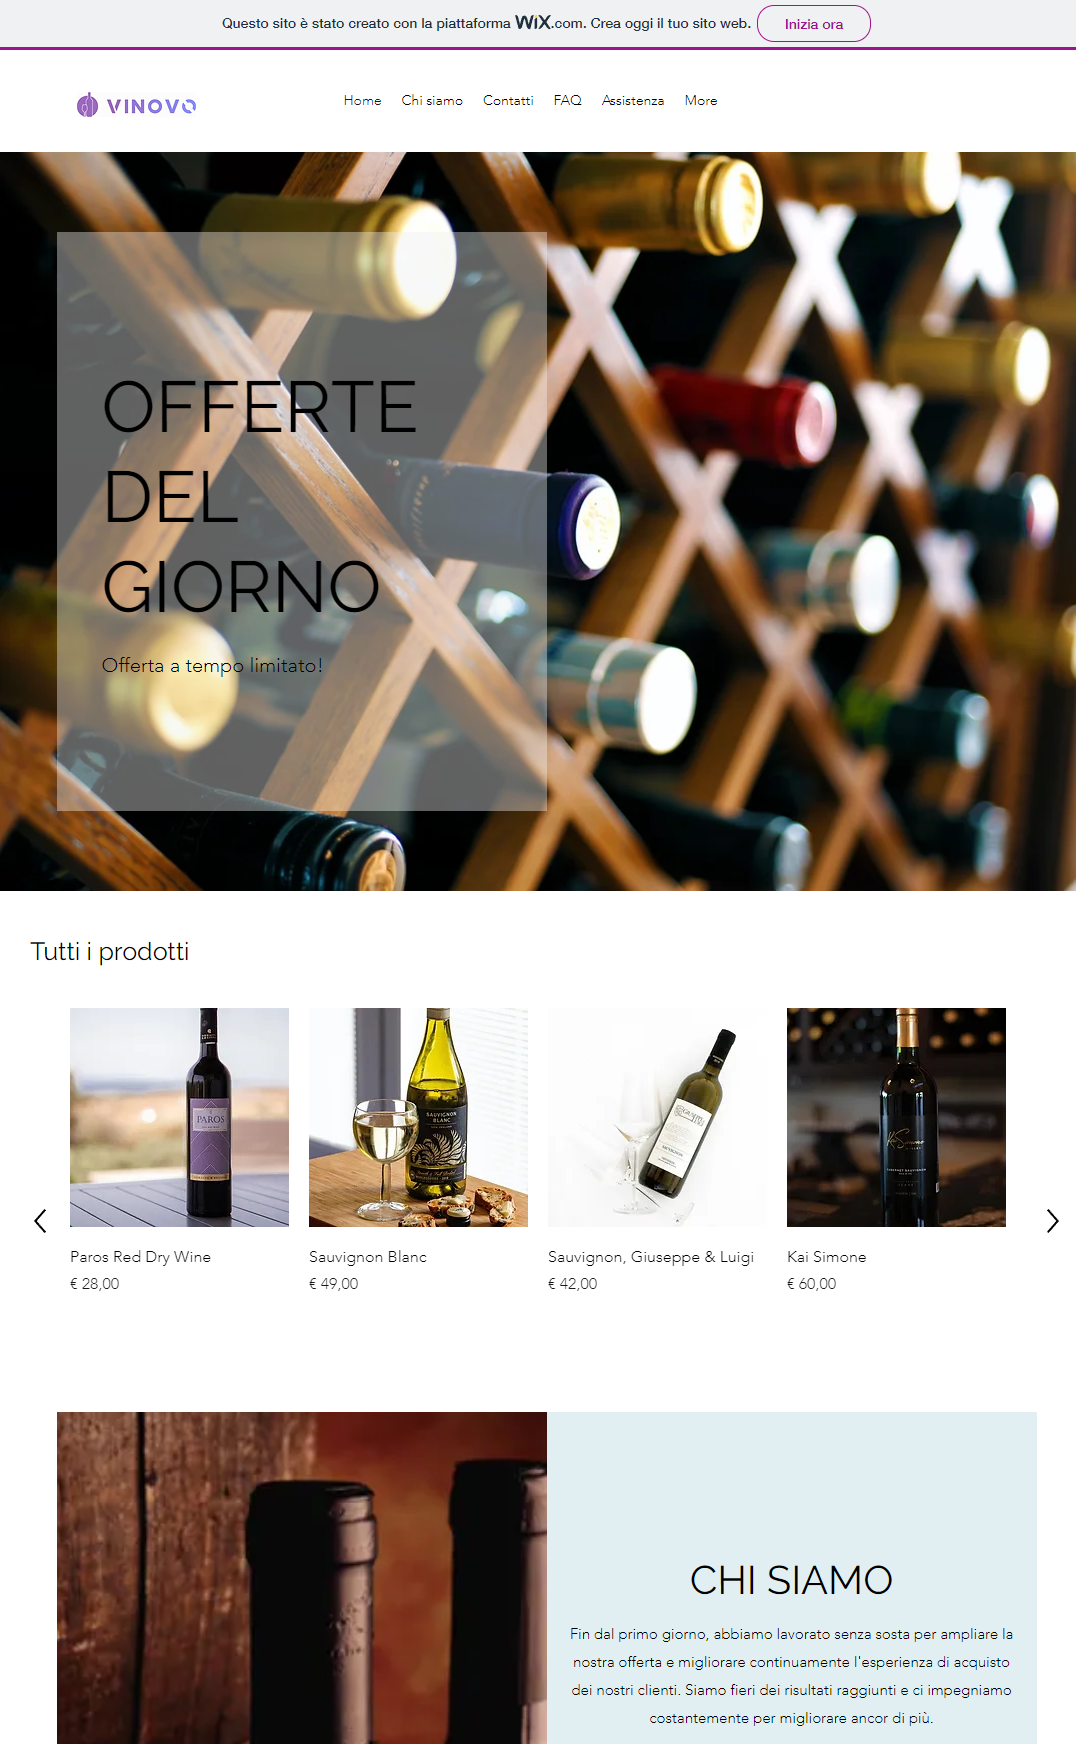
\includegraphics[width=.93\textwidth]{images/sito.png}}
\end{center}

\end{document}